\documentclass[a4paper,titlepage,fleqn,12pt]{article}

\usepackage[utf8]{inputenc}
\usepackage[T1]{fontenc}
\usepackage[english]{babel}
\usepackage{color}
\usepackage{float}
\usepackage{fancyvrb}
\usepackage{amssymb}
\usepackage{amsmath}
\usepackage{listings}

\usepackage{comment}

\usepackage{graphicx}
\usepackage{ulem}
\usepackage{pdfpages}

\DeclareGraphicsExtensions{.png}

\definecolor{dkgreen}{rgb}{0,0.45,0}
\definecolor{gray}{rgb}{0.5,0.5,0.5}
\definecolor{mauve}{rgb}{0.30,0,0.30}

\lstset{frame=tb,
  language=Java,
  aboveskip=3mm,
  belowskip=3mm,
  showstringspaces=false,
  columns=flexible,
  basicstyle={\small\ttfamily},
  numbers=left,
  numberstyle=\footnotesize,
  keywordstyle=\color{dkgreen}\bfseries,
  commentstyle=\color{dkgreen},
  stringstyle=\color{mauve},
  frame=single,
  breaklines=true,
  breakatwhitespace=false
  tabsize=1
}


\begin{document}

\begin{titlepage}
	\begin{center}
	
\includegraphics[scale=1.5,page=7]{sdu_logos.pdf}~\\[0.5cm]
	\textsc{\Large{SydDansk Universitet - Mærsk Merkini Møller Institutet}} \\[0.2cm]
	\rule{12cm}{1pt} \\[0.4cm]
	{ \huge \bfseries Interaktion og interaktions design, efterår 14, Projekt del 1 \\[0.4cm] }
	\rule{12cm}{1pt} \\[1.5cm]
	
	\begin{minipage}{0.4\textwidth}
		\begin{flushleft} \large
			\textit{Author:}\\
			Morten Rovelt Hansen\\
			Brian Pedersen\\
			Steven Gøhler\\
		\end{flushleft}
	\end{minipage}
	\begin{minipage}{0.4\textwidth}
		\begin{flushright} \large
			\textit{Supervisor:} \\
			Jess Uhre Rahbek
		\end{flushright}
	\end{minipage}
	
	\vfill
	
	{\large Oktober 10, 2014}
	\end{center}
	\newpage
\end{titlepage}

\section{Table Of Contents}
\tableofcontents
\newpage

\section{Test af prototyper}

\subsection{Prototype 1}

\begin{figure}[H]
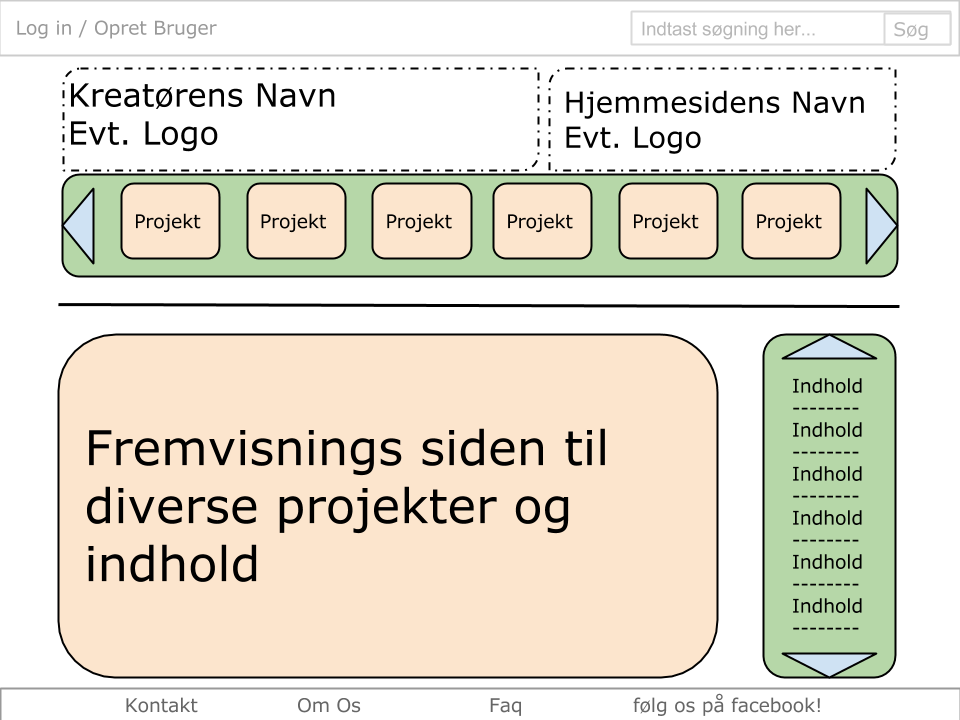
\includegraphics[width=\textwidth]{hjemmesidedesign1.png}

\end{figure}

\subsubsection{Fordele}

\begin{itemize}
\item Let tilgængelig søgefunktion.
\item Det fremgår tydeligt hvis portfolie man er inde på.
\item Overskueligt og nemt at tilgå diverse funktioner.
\end{itemize}

\subsubsection{Ulemper}
\begin{itemize}
\item Svært at finde et specifikt billede i et projekt med mange billeder. 
\item Forvirrende med både horisontale og vertikale lister
\item Manglende information om indholdet i projekterne
\end{itemize}

\subsection{Prototype 2}

\begin{figure}[H]
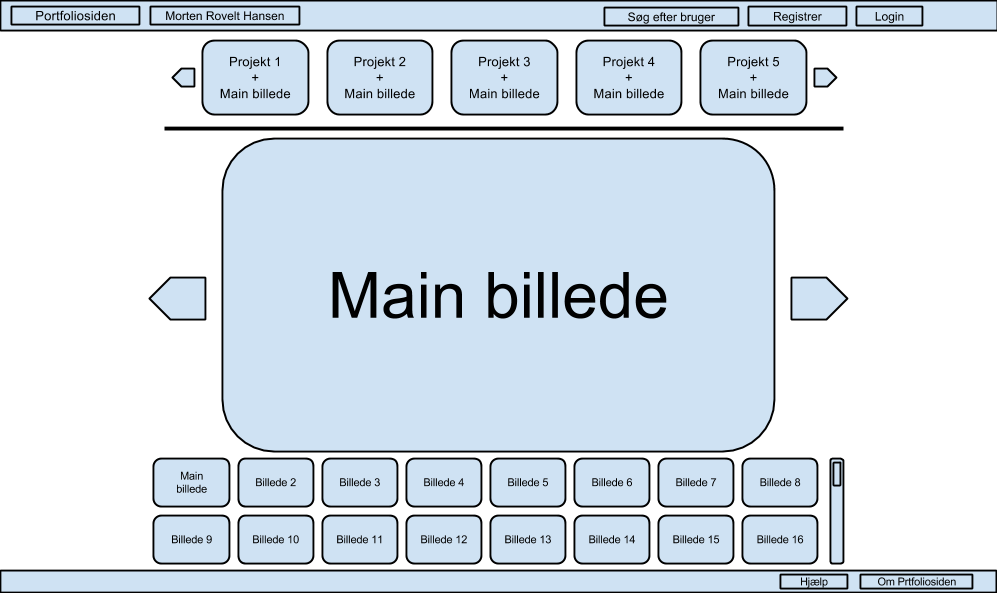
\includegraphics[width=\textwidth]{Prototype_1_not_logged_in.png}
\end{figure}

\begin{figure}[H]
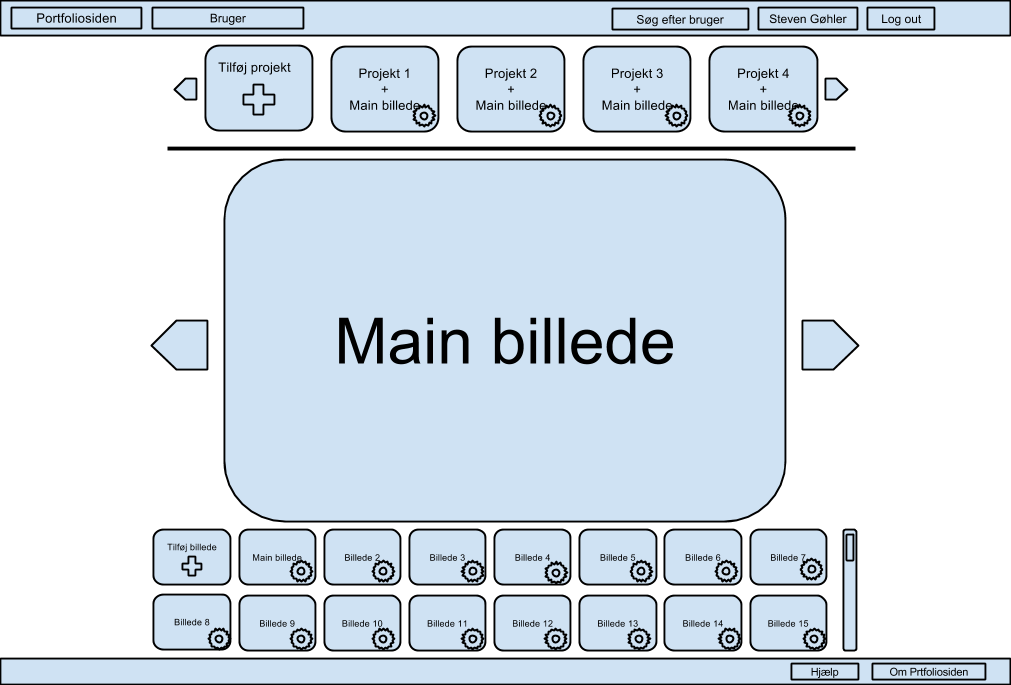
\includegraphics[width=\textwidth]{Prototype_1_logged_in.png}
\end{figure}

\subsubsection{Fordele}
\begin{itemize}
\item Let tingængelig søgefunktion
\item Simpelt og overskueligt
\item Nemt at tilføje/slette projekter og billeder
\end{itemize}

\subsubsection{Ulemper}
\begin{itemize}
\item For mange elementer på skærmen af gangen
\item Scroll bar bliver muligvis et problem
\item Manglende infirmation om inholdet i projekterne
\end{itemize}

\subsection{Prototype 3}

\begin{figure}[H]
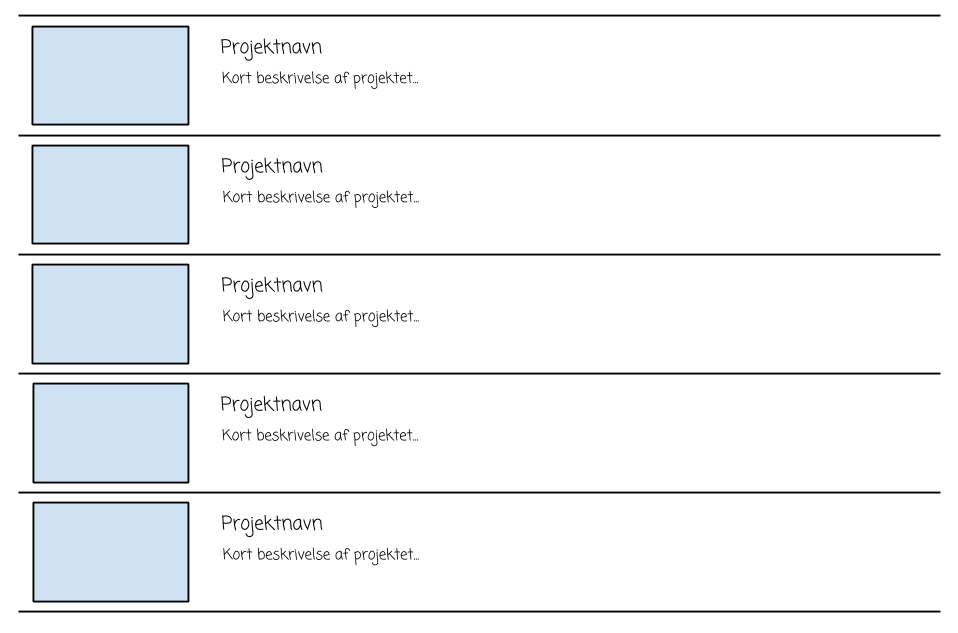
\includegraphics[width=\textwidth]{Sketch2_1.png}
\end{figure}

\begin{figure}[H]
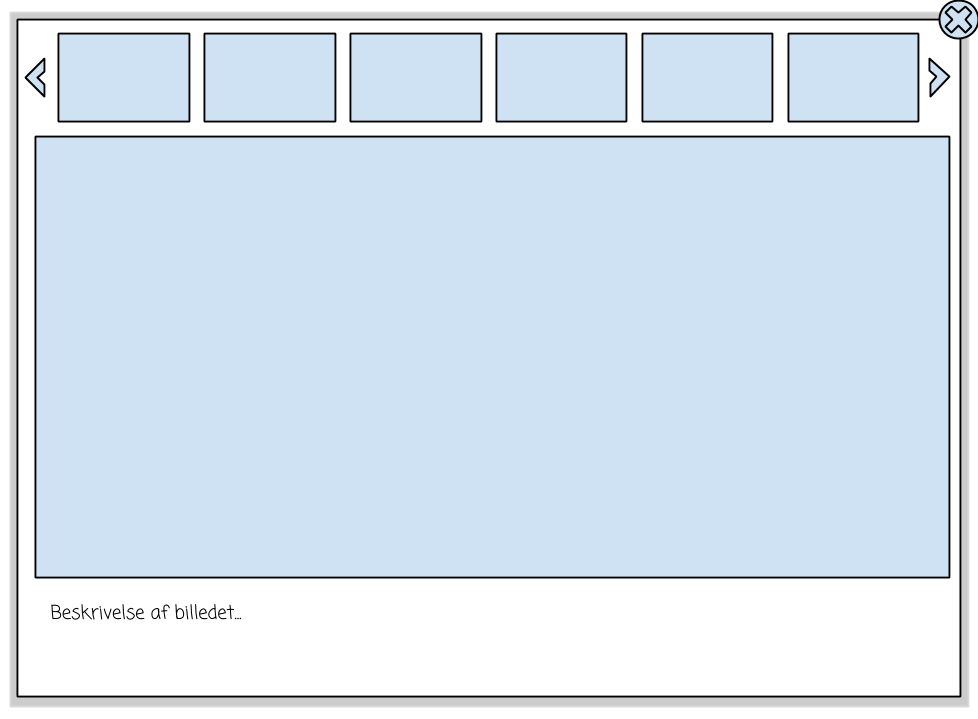
\includegraphics[width=\textwidth]{Sketch2_2.png}
\end{figure}

\subsubsection{Fordele}
\begin{itemize}
\item God information omkring projekterne
\item Der er et minimum af elementer på siderne af gangen
\end{itemize}

\subsubsection{Ulemper}
\begin{itemize}
\item Det er ikke nemt at tilgå et nyt projekt
\end{itemize}

\section{Valg af design}

Vi har valgt Prototype 3, vi vil dog impementere tandhjulene fra Prototype 2 som gør det redigere i ens projektor. Tilmed vil vi også implementere tilføj billede/projekt fra Prototype 2 når man er logget ind på sin egen bruger. Vi vil også implementere de to bokse med Kreatørens navn og Hjemmesidens navn fra prototype 1, så det bliver let at se hvis portfolie man er inde på. Header og footer fra bliver også tilføjet til prototypen, i stil med prototype 1/2.


\end{document}